\documentclass[12pt]{article}

\setlength\parindent{0pt}

\usepackage[english]{babel}
\usepackage{graphicx}
\usepackage{amsmath}
\usepackage{tikz}
\usepackage{hyperref}
\usepackage{graphicx}
\usepackage[a4paper, total={}]{geometry}
\setlength{\headsep}{5pt}
\setlength{\parskip}{1em}
\usepackage{listings}
\usepackage{extarrows}
\newtheorem{definition}{Definition}

\definecolor{pblue}{rgb}{0.2,0.2,0.7}
\definecolor{pgreen}{rgb}{0,0.5,0}
\definecolor{pred}{rgb}{0.7,0.2,0.2}
\definecolor{pgrey}{rgb}{0.46,0.45,0.48}

\lstset{
	language=Java,
	showstringspaces=false,
	columns=flexible,
	basicstyle={\small\ttfamily},
	numbers=none,
	numberstyle=\tiny\color{gray},
	keywordstyle=\color{blue},
	commentstyle=\color{pgreen},
	stringstyle=\color{mauve},
	breaklines=true,
	breakatwhitespace=true,
	tabsize=3
}

\hbadness=10000

\usetikzlibrary{automata, positioning, arrows}

\tikzset{
	->,
	node distance=3cm,
	initial text=$ $,
}

\title{\vspace{-20px}Incremental code clone management in modern IDE environments}

\author{Jakob Konrad Hansen}

\date{Last updated \today}

\begin{document}
\maketitle


\tableofcontents

\newpage

\section{Introduction}

Refactoring is the process of restructuring source code in order to improve the internal behavior
of the code, without changing the external behavior\cite[9]{fowlerrefactoring}.
Refactoring on source code is often performed in order to eliminate instances of bad
design quality in code, otherwise known as code smells.

A study conducted by Diego Cedrim et al. has shown that while developers tend to refactor
smelly code, they are rarely successful at eliminating the smells they are
targeting\cite{Rohit_Gheyi_Impact}. A large portion of refactorings even tend to make the
code quality worse. Therefore, automated tools to help developers make better refactorings
and perform code analysis is an important field of research.

Duplicated code is a code smell which occurs in practically every large software project.
Code clone analysis has recently become a highly active field of research and many tools
have been developed to detect duplicated code\cite[7]{Inoue_introduction_to_cc}. However,
few of these have the capability of detecting intricate types of duplicated code and
managing them in a real-time IDE environment.

This thesis will present a tool and possibly techniques for clone detection and management
in real-time, for usage in modern IDE environments. The thesis will explore the topics
such as finding and managing clones in real-time, incremental analysis of source code and
providing clone management and refactoring tools in a modern IDE environment.

\section{Background}

\subsection{Software quality and duplicated code}

Software quality is hard to define. The term ``quality'' is ambiguous and is in the case
of software quality, multidimensional. Quality in itself has been defined as ``conformance
to requirements'' \cite[8]{crosby1980quality}. In software, the simplest measure of
``conformance to requirements'' is a lack of bugs. However, software
quality is often measured in other metrics, including metrics which are not directly
related to functionality\cite[29]{MetricsAndModelsInSoftwareQuality}. These metrics
often include maintainability, analyzability and changeability.

These metrics are affected negatively by duplicated code, code which is more or less
copied to different locations in the source code. Multiple studies have shown that
software projects typically contains $10-15\%$ duplicated code\cite{CloningByAccident}.
Therefore, research into tools and techniques which can reduce duplicated code will be of
benefit to almost all software.

As stated, duplicated code damages software quality in software projects. Duplicated code
can lead to a plethora of antipatterns, and will often lead to an increase in technical
debt. The ``Shotgun-Surgery''\cite[66]{fowlerrefactoring} antipattern occurs when a
developer wants to implement a change, but needs to make the same change in multiple
locations for the change to take effect. This is a typical situation which slows down
development and reduces maintainability when a software project contains a lot of
duplicated code.

\subsection{Code clones}

Duplicated code is often described as ``code clones''.

\begin{definition}[Code snippet]
	A code snippet is a piece of source code in a larger software system.
\end{definition}

\begin{definition}[Code clone]
	A code clone is a code snippet which is equal to or similar to another code snippet. The two
	code snippets are both code clones, and together they form a code clone pair.
\end{definition}

\subsubsection{Clone relation}

The clone relation is a relation between code snippets which defines pairs of clones.
The clone relation is reflexive and symmetric, but not always transitive. The transitive
property depends on the threshold for similarity when identifying code clones. Given

$$a \xleftrightarrow{clone} b \xleftrightarrow{clone} c$$


where $a,b,c$ are code snippets and $\xleftrightarrow{clone}$ gives the clone relation, $a$ is
a clone of $b$, but not necessarily similar enough to be a clone of $c$, depending on the
threshold for similarity.
\subsubsection{Code clone types}

Code clones are generally classified into four types\cite{Inoue_introduction_to_cc}. The
types classify code snippets as code clones with an increasing amount of leniency.
Therefore, Type-1 code clones are very similar, while Type-4 clones are not necessarily
similar at all. However, all code clones have the same functionality, it is the syntactic
and structural differences which distinguishes the types. The set of code clones
classified by a code clone type is also a subset of the next type, meaning all Type-1
clones are also Type-2 clones, but not vice versa.

The code clone types are defined as follows:

\textbf{Type-1} clones are syntactically identical. The only differences allowed are elements
without meaning, like comments and white-space. Example:

\begin{lstlisting}[frame=single]
// Clone 1
for (int i = 0; i < 10;   i++) {
    print(i);
}

// Clone 2
for (int i = 0; i < 10; i++) {
    // A comment without meaning
    print(i);
}

\end{lstlisting}

\textbf{Type-2} clones are structurally identical. Possible differences include
identifiers, literals and types. Type-2 clones are relatively easy to detect by
consistently renaming identifiers and literals.\cite[2]{Zibran_real_time_search} Example:

\begin{lstlisting}[frame=single]
// Clone 1
for (int i = 0; i < 10; i++) {
    print(i);
}

// Clone 2
for (int j = 1; j < 10; j++) {
    print(j);
}
\end{lstlisting}

\textbf{Type-3} clones are required to be structurally similar, but not equal. Differences
include statements which are added, removed or modified. This clone type relies on a
threshold $\theta$ which determines how structurally different snippets can be to be
considered Type-3 clones\cite{Inoue_introduction_to_cc}. The granularity for this
difference could be based differing tokens, lines, etc. Detecting this type of clone is
hard. Example:

\begin{lstlisting}[frame=single]
// Clone 1
for (int i = 0; i < 10; i++) {
    print(i);
}

// Clone 2
for (int i = 0; i < 10; i++) {
    print(i);
    int x = 10;
}
\end{lstlisting}

In this example there is a one line difference between the two snippets, so if $\theta
	\geq
	1$, the two snippets would be considered Type-3 clones.

\textbf{Type-4} clones have no requirement for syntactical or structural similarity.
Therefore, the only requirement is equal functionality. Detecting this type of clone is
very challenging, but attempts have been made using program dependency
graphs\cite{SeedType4Detection}. The following example shows two code snippets which have
no clear syntactic or structural similarity, but is functionally equal:

\begin{lstlisting}[frame=single]
// Clone 1
print((n*(n-1))/2)

// Clone 2
int sum = 0;
for (int i = 0; i < n; i++) {
    for (int j = i+1; j < n; j++) {
        sum++;
    }
}
print(sum);
\end{lstlisting}

In this example there is no clear similarity in the two snippets, but they have the same
functionality.

Type-1 clones are often referred to as ``exact'' clones, while Type-2 and Type-3 clones
are referred to as ``near-miss'' clones\cite[1]{Zibran_real_time_search}.

\subsubsection{Code clone detection process and techniques}

\textbf{The Code clone detection process} is generally split into (but is not limited to)
a set of steps to identify clones\cite{Inoue_introduction_to_cc}. This
process is often a pipeline of input-processing steps before finally comparing fragments
against each other and filtering. The steps are generally as follows:

\begin{enumerate}
	\item \textbf{Pre-processing}: Removing uninteresting parts which we do not want to
	      check for clones, for example generated code. Then partition code into a set of
	      fragments, depending on granularity. Granularity could be entire files, methods or lines.
	\item \textbf{Transformation}: Transform fragments into an intermediate representation.
	      \begin{enumerate}
		      \item Extraction: Transform source code into the input for the comparison
		            algorithm. Can be tokens, AST, dependency graphs, suffix tree, etc.
		      \item Normalization: Optional step which removes superficial differences such as
		            comments, whitespace and identifier names. Often useful for identifying type-2
		            clones.
	      \end{enumerate}
	\item \textbf{Match detection}: Perform comparisons which outputs a set of
	      candidate clone pairs.
	\item \textbf{Formatting}: Convert candidate clone pairs from the transformed
	      code back to clone pairs in the original source code.
	\item \textbf{Post-processing/Filtering}: Ranking and filtering manually or with
	      automated heuristics
	\item \textbf{Aggregation}: Optionally aggregating sets of clone pairs into clone classes
\end{enumerate}

Not all clone detection techniques will necessarily follow all these steps.

\textbf{Matching techniques} are techniques which can be applied to match source-code to
detect clone-pairs, with various advantages and disadvantages. The matching technique will
also require specific pre-processing to be done in the earlier steps, for example creating an
AST. Some of the most explored techniques are as follows\cite{ComparisonAndEvaluationOfTechniques}:

\textit{Text-based} approaches do very little processing on the source code before
comparing. Simple techniques such as fingerprinting or incremental hashing have been used
in this approach. Dot plots have also been used in newer text-based approaches, placing
the hashes of fragments in a dot plot for use in comparisons.

\textit{Token-based} approaches transform source code into a stream of tokens, similar to
lexical scanning in compilers. The token stream is then scanned for duplicated
subsequences of tokens. Since token streams can easily filter out superficial differences
such as whitespace, indentation and comments, this approach is more robust to such
differences. Concrete names of identifiers and values can be abstracted away when comparing
the token-stream, therefore Type-2 clones can easily be identified. Type-3 clones can also
be identified by comparing the fragments tokens and keeping clone pairs with a lexical
difference lower than a given threshold. This can be solved with dynamic
programming\cite{BakerSparseDynamicProgramming}. A common approach to detect clones using
token-streams is with a suffix-tree. A suffix-tree can solve the \textit{Find all maximal
	repeats} problem efficiently, which in essence is the same problem as finding clone pairs.
This algorithm can also be improved to use a suffix-array instead, which requires less
memory.

\textit{Syntactic} approaches transform source code into either concrete syntax trees or
abstract syntax trees and find clones using either tree matching algorithms or structural
metrics. For tree matching, the common approach is to find similar subtrees in the tree,
which are then deemed as clone pairs. One way of finding similar subtrees is to hash
subtrees into buckets and compare them with a tolerant tree matching algorithm. Variable
names, literal values and other source may be abstracted to find Type-2 clones more
easily. Metrics-based techniques gather metrics for code fragments in the tree and uses
the metrics to determine if the fragments are clones or not. One way is to use
fingerprinting functions where the fingerprint includes certain metrics, and compare the
fingerprints of all fragments to find clones.

\textit{Chunk-based} approaches decompose chunks of source code into signatures which are
compared. Chunk-size is based on selected granularity, which can be functions, blocks,
etc. Signatures can for example be based on some software metrics. Machine learning has
been used in this approach using methods as chunks and token-frequency within the method
as signature. A Deep Neural Network trained on this data can then be used to classify two
chunks as clone or non-clone.

\textit{Hybrid} approaches combine multiple approaches in order to improve detection. For
example Zibran et al.\cite{Zibran_real_time_search} developed a hybrid algorithm
combining both token-based suffix trees for Type-1 and Type-2 clone detection, with
a k-difference dynamic programming algorithm for Type-3 clone detection.

\subsubsection{Code clone merging techniques}

Automated merging of code clones is a mostly unexplored area of research, but some work has
been done.

Yoshiki Higo\cite{RefactoringOrientedClonesAndMerging} introduced the notion of a
\textit{refactoring oriented} clone in object-oriented languages, which means stripping
parts of clones to make them easier to automatically merge. With these clones they boiled
the merging process down to three cases:

\textbf{Case 1:} If clones are in the same class, they can be merged as a new method.

\textbf{Case 2:} If clones inherit from the same class, they can be merged as a new
method in the common super-class.

\textbf{Case 3:} If clones are scattered between unrelated classes, a new class can be
created where the method is merged. If the classes containing the clone do not inherit
from other classes, the classes can inherit from the new class.

They also introduced metrics for use in determining how merging should be done.

\subsubsection{IDE-based clone management}

Developers are not always aware of the creation of clones in their code. Clone aware
development means having clone management as a part of the software development
process. Since code clones can be hard to keep track of and manage, tools which help
developers deal with clones are useful. However, Mathias Rieger et al. claims that
a problem with many detection tools is that the tools ``report large amounts data that must
be treated with little tool support''\cite[1]{InsightsSystemWideDuplication}. Detecting
and eliminating clones early in their lifecycle is therefore vital for the developer to
have success in managing their clones.

There are many existing clone management tools, however the most useful tools for clone
aware development are the tools which are integrated into an IDE and offer services to the
programmer while developing in real-time.

The IDE-based tools which exist can be categorized as
follows\cite[8]{Udding_Towards_Convenient_Management}:

\begin{itemize}
	\item\textit{Copy-paste-clones:} This category of tools deals only with code snippets which are
	copy-pasted from another location in code. These tools therefore only track clones which
	are created when copy-pasting, and does not use any other detection techniques. Therefore,
	this type of tool is not suitable for detecting clones which are made accidentally, since
	developers are aware that they are creating clones when pasting already existing code
	snippets.

	\item\textit{Clone detection and visualization tools:} This category of tools has more
	sophisticated clone detection capabilities and will detect code clones which occur
	accidentally.

	\item\textit{Versatile clone management:} This category of tools covers tools which provide more
	services than the above. Services like refactoring and simultaneous editing of clones fall
	under this category.
\end{itemize}

There are a few existing IDE-tools which have seen success in real-time detection of clones:

\begin{itemize} \item Minhaz et al. introduced a hybrid technique for performing real-time
	      focused searches, i.e. searching for code clones of a selected code snippet. This
	      technique can also detect Type-3 clones\cite{Zibran_real_time_search}. This technique
	      was later used in the tool
	      \textit{SimEclipse}\cite{Udding_Towards_Convenient_Management}. Since this tool can
	      only detect clones of a code snippet which the developer actively selects, this tool
	      is not well suited for finding accidental clones.

	\item Another tool, SHINOBI can detect code clones in real-time without the need of
	      the developer to select a code snippet, however it can only detect type-1 and
	      Type-2 code clones. The tool uses a token-based suffix array index approach to detect
	      clones incrementally\cite{SHINOBI}.

	\item The modern IDE IntelliJ has a built-in duplication detection and
	      refactoring service, it is able to detect type-1 and (some) type-2 code clones
	      at a method granularity and refactors by replacing one of the clones with a
	      method call to the other.
\end{itemize}


\subsection{Incremental editing and analysis}

While writing code, programmers usually only edit small portions of text at a time. One
``edit'' will therefore only affect small parts of the internal representations of the
code which most tools use to perform analysis. Reusing parts of this representation would
therefore be faster and allow programming tools to scale better.

\subsubsection{Incremental parsing}

Incremental parsing is the process of reparsing only parts of a syntax tree whenever an
edit is performed. The motivation behind incremental parsing is to have a readily
available syntax tree after every edit, while doing as little computing as possible to
build it.

Ghezzi and Mandrioli first introduced the notion of incremental parsing, and introduced an
incremental parser for LR $\land$ RL grammars. However, they were aware that this
algorithm was both slow and didn't allow expressive enough
grammars.\cite{incrementalparsing}

Tim A. Wagner\cite{PracticleAlgorithmsForIncremental} and his research group later
published a large work on incremental software development environments, presenting many
novel algorithms and techniques for incremental tooling in programming environments.

``Tree-sitter'' is a parser generator tool which specializes in incremental parsing.
Inspired by Wagner's work, it supports incremental parsing, error recovery and querying
for specific nodes and subtrees.\cite{treesitter} These features combined allow
Tree-sitter to become a powerful tool for analysis and has been used for editor features
such as syntax-highlighting, refactoring and code navigation.

\subsubsection{Incremental clone detection}

In order to incrementally detect code clones, an algorithm which first calculates the
initial code clones is run, and for successive revisions of the source code, this list is
incrementally updated, more efficiently than the initial run. Different approaches have
been used to accomplish this.


Göde and Koschke\cite{GodeIncrementalCloneDetection} proposed the first incremental clone
detection algorithm. The algorithm employs a generalized suffix tree in which the amount
of work of updating is only dependent on the size of the edited code. This approach is
limited in scalability, as generalized suffix trees require a substantial amount of
memory.

Nguyen et al. showed that an AST-based approach utilizing ``Locality-Sensitive Hashing''
can detect clones incrementally with high precision, in real-time ($< 1$ second).

Hummel et al.\cite{IndexBasedIncrementalCloneDetection} presented the first incremental
and scalable clone detection technique for Type-1 and Type-2 clones. This approach
utilizes a custom ``clone index'' data structure which can be updated efficiently. The
implementation of this data structure is similar to that of an inverted index.

More recently, Ragkhitwetsagul and Krinke\cite{SiameseScalableAndIncrementalClone}
presented the tool ``Siamese'', which uses a novel approach of having multiple
intermediate representations of source code to detect a high number of clones with
support for incremental detection. The tool can detect up to Type-3 clones, but will only
give clones based on queries given to it by the user. 

\subsection{The Language Server Protocol}

The Language Server protocol (LSP) is a protocol which specifies interaction between a
client (IDE) and server in order to provide language tooling for the client. The goal of
the protocol is to avoid multiple implementations of the same language tools for every
IDE and every language. Servers which implement LSP will be able to offer IDE's
code-completion, diagnostics, go-to-definition and more. LSP also specifies generic
code-actions and commands, which the LSP server provides to the client in order to perform
custom actions defined by the server.

Figure \ref{fig:lspcommunication} shows a sample interaction between client and server
using LSP. The client sends requests to a server in the form of JSON-RPC messages, and the
server sends a corresponding response, also in the form of JSON-RPC messages.

\begin{figure}
	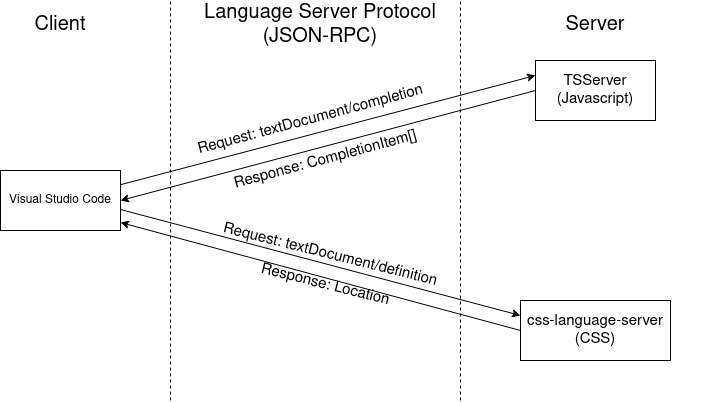
\includegraphics[width=\textwidth]{images/lspcommunication.png}
	\caption{Example client-server interaction using LSP}
	\label{fig:lspcommunication}
\end{figure}

\section{The way forward}

This thesis will present and evaluate a tool which provides clone management
capabilities in a real-time IDE environment. The main goal will be to create a tool which
fits well into the development cycle and works in a real-time IDE environment. Areas of
focus will therefore be:

\begin{itemize}
	\item Code clone detection and refactoring of code clones
	\item Real-time / Incremental detection and management of code clones
	\item IDE tooling and IDE agnostic tooling like LSP
	\item Possibly clone ranking, determining which clones should be kept.
\end{itemize}

\subsection{LSP for IDE-based clone management}

The tool will give programmers the ability to manage clones in their IDE. We will utilize
many feature of LSP, especially code-actions, in order to provide functionality for clone
management to any editor which implements LSP.

The following user stories shows how interaction with the LSP server will work.

\begin{itemize}
	\item A programmer wants to see code clones for a single file, the
	      programmer opens the file in their IDE and is displayed diagnostics in the code
	      wherever there are detected clones.

	\item A programmer wants to see all code clones for the current project. The
	      programmer opens the IDE's diagnostic view and will see all code clones detected
	      as diagnostics there. The diagnostic will contain information like where the clone
	      exists, and percentage of duplicated code.

	\item A programmer wants to jump to the corresponding match of a code clone in their
	      editor. The programmer moves its cursor to the diagnostic and will see a list of
	      the matching code clones. The programmer will select the wanted code clone which
	      will move the cursor to the file and location of the selected code clone.

	\item A programmer wants to merge a code clone pair. The programmer moves their cursor
	      to one of the code clones, invokes a request to see code actions, and invokes one
	      of the ``Merge code clone with strategy x`` actions. The strategies presented to
	      the user is dependent on the context of the code clone pair, the programmer will
	      only see the useful / realizable merging strategies.
\end{itemize}

The interaction with the LSP server will depend on the client's implementation of LSP. If
the LSP client is limited in its capabilities, meaning it doesn't implement the entire
protocol, the tool will be limited in how the programmer can interact with it.

\subsection{Architecture of tool}

Figure \ref{fig:architecture} shows the architecture of the tool. The server communicates
with the IDE and delegates the work of managing clones to the detection engine and the
merge engine. The tool also stores an index of all source code files in the current project.

\subsection{Exploring clone management techniques}

During development of the tool, different techniques for detecting and merging clones will
be explored. The goal will be to find a fitting technique for both detecting and merging
clones in a real-time IDE environment.

Detection techniques explored will include:

\begin{itemize}
	\item A fully incremental version of Zibran et al. hybrid
	      algorithm\cite{Zibran_real_time_search}
	\item AST-based technique with incremental parsing. Using Tree-sitter to parse and an
	      incremental detection algorithm to detect clones.
\end{itemize}

Merging techniques explored will include:

\begin{itemize}
	\item Refactoring-oriented clone merging\cite{RefactoringOrientedClonesAndMerging}
\end{itemize}

\begin{figure}
	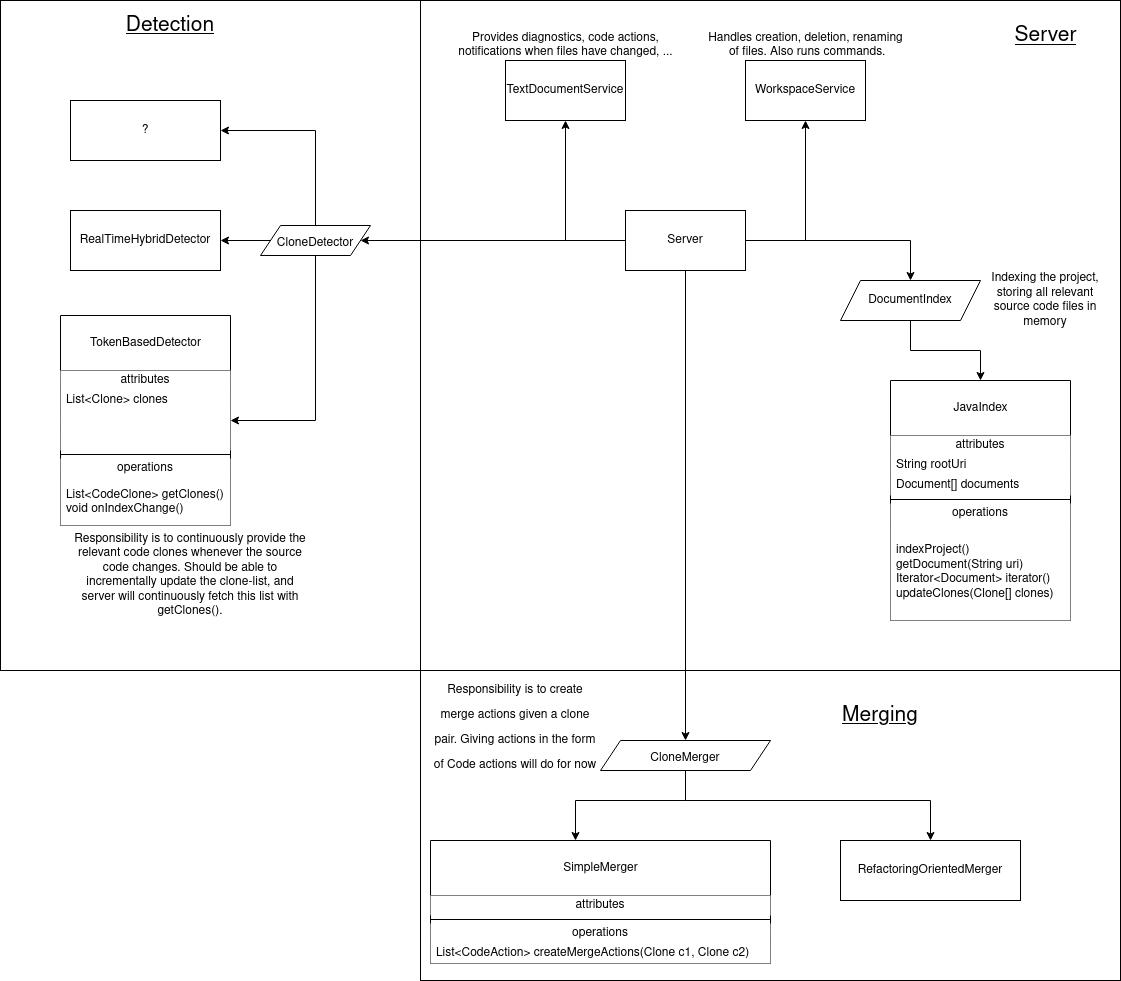
\includegraphics[width=\textwidth]{images/ToolArchitecture.png}
	\caption{Tool architecture}
	\label{fig:architecture}
\end{figure}

The tool will be modular in how techniques are applied for clone management. This
means that the tool will be capable of plugging in different detection engines, merging
engines and file indices. This will be used extensively in our research in order to test
multiple techniques for detection and merging.

\subsection{Evaluation}

We will evaluate this tool based on different criteria, which combined will provide a
basis for evaluating the tool as a whole.

Since the tool is focused on efficient detection and management of code clones, real-time
performance of the tool will be a high priority in its evaluation. The tool will implement
different techniques of detecting and merging clones. These will be empirically compared
against each other. The tool will also be evaluated against existing tools empirically. We
will utilize BigCloneBench\cite{BigCloneBench} to evaluate detection techniques, by
running our detection techniques in a standalone mode. We will distinguish between initial
detection and incremental detection when evaluating.

The tool will also be evaluated based on its effectiveness in managing clones. Can we
determine if this tool is better than existing tools at managing or eliminating clones in
the software development cycle?

Finally, we will evaluate if LSP is a suitable tool for use in clone management and
refactoring in general. Can LSP provide all the features one would want in a modern
analysis and refactoring tool? What is missing, and how could the LSP protocol be extended
in order to facilitate this? We believe that if LSP is an appropriate tool to use for
clone management, LSP will also be an appropriate tool for refactoring tools in general.

\newpage
\bibliography{refs}
\bibliographystyle{plain}

\end{document}
